\documentclass[14pt]{beamer}
\usepackage[english,russian]{babel}
\usepackage{indentfirst}
%\usepackage[dvipsnames]{xcolor}
\usepackage{amsfonts} 
\usepackage{amsmath, etoolbox}
\usepackage{graphicx}
\usepackage{float}
\graphicspath{{figure/}}
\DeclareGraphicsExtensions{.png,.jpg}

\usepackage{fancyhdr}
\pagestyle{fancy}
\fancyfoot{} 

\usepackage{listings}

\usetheme{AnnArbor}

\begin{document}
	\begin{frame}
		\title{Параллельные структуры данных}
		\author{Дамаскинский Константин}
		\titlepage
	\end{frame}

	\begin{frame}{Что требуется?}
		\begin{itemize}
			\item Контейнеры
			\begin{enumerate}
				\item Список (стек, очередь)
				\item Множество
			\end{enumerate}
		\end{itemize}
	\end{frame}

	\begin{frame}{Модели доступа}
		\begin{itemize}
			\item Single producer, multiple consumers
			\item Multiple producers, multiple consumers
			\item Single consumer, multiple producers
		\end{itemize}
	\end{frame}

	\begin{frame}{Параллельное выполнение операций}
		\begin{itemize}
			\item Чтение
			\begin{enumerate}
				\item Чтение разрешено
				\item Изменение запрещено
			\end{enumerate}
			\item Изменение
			\begin{enumerate}
				\item Чтение запрещено
				\item Изменение запрещено
			\end{enumerate}
		\end{itemize}
	
		От метода синхронизации доступа зависит, \textbf{на какую составляющую контейнера} накладываются указанные ограничения
	\end{frame}

	\begin{frame}
		\begin{center}
			\Large{Множество на связном списке}
		\end{center}
	\end{frame}
	
	\begin{frame}{Coarse-grained synchronization}
		\begin{itemize}
			\item Блокирование доступа ко всему контейнеру при чтении (поиске элемента)
			\item Блокирование доступа ко всему контейнеру при записи
			\item Хорошо работает при небольшом количестве параллельных читателей
			\item Наименее эффективный метод синхронизации
		\end{itemize}
	\end{frame}

	\begin{frame}{Fine-grained synchronization}
		\begin{itemize}
			\item Блокирование доступа к каждому элементу списка по отдельности \textbf{по достижении}
			\item Позволяет итерироваться нескольким потокам одновременно
			\item Необходимо сначала получать доступ к очередному интересующему элементу, а затем освобождать доступ к текущему
		\end{itemize}
	\end{frame}

	\begin{frame}{Fine-grained synchronization}
		\begin{figure}
			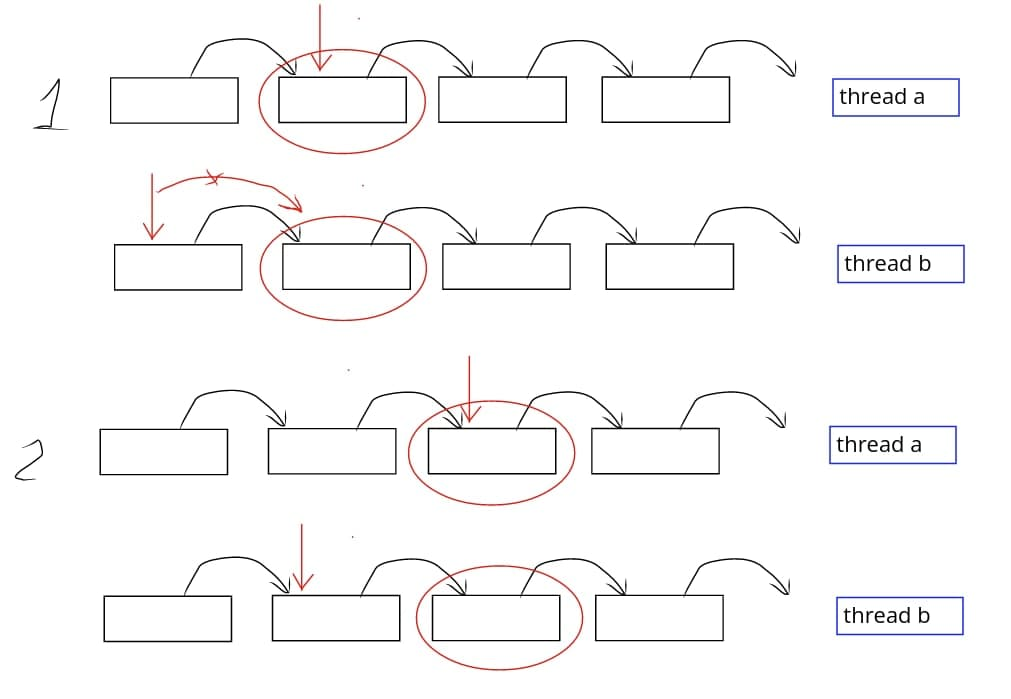
\includegraphics[scale=0.33]{fine-grained}
		\end{figure}
	\end{frame}

	\begin{frame}{Optimistic synchronization}
		\begin{itemize}
			\item \textbf{Проблема fine-grained sync.} Поток, который читает второй элемент, заблокирует поток, который читает пятый элемент
			\item \textbf{Решение.} Контейнер не блокируется при поиске нужного элемента при чтении
			\item После нахождения требуемого элемента проверяется производится блокирование элемента. Затем проверяется, изменился ли элемент между моментом обнаружения и блокировки. Если не изменился, чтение успешно завершается
		\end{itemize}
	\end{frame}

	\begin{frame}{Lazy synchronization}
		\begin{itemize}
			\item Трудоёмкие операции выполняются в ленивом режиме. Конкретно: при удалении взводится флаг ``удалён'', а физическое извлечение из памяти производится позже (после снятия блокировки)
		\end{itemize}
	\end{frame}

	\begin{frame}
		\begin{center}
			\Large{Lock-free очереди}
		\end{center}
	\end{frame}

	\begin{frame}{Lock-free и wait-free}
		\begin{itemize}
			\item \textbf{Lock-free структура данных}  гарантирует, что \textbf{некоторый} поток закончит выполнение операции над объектом за конечное число шагов \textit{вне зависимости от результата работы других потоков} (даже если эти другие потоки завершились крахом)
			
			\item \textbf{Wait-free структура данных}  гарантирует, что \textbf{все} потоки закончат выполнение операции над объектом за конечное число шагов
		\end{itemize}
	\end{frame}

	\begin{frame}{Lock-free. Как это работает?}
		\begin{itemize}
			\item Отказ от примитивов синхронизации
			\item Использование атомарных операций
			\begin{enumerate}
				\item CAS -- compare and swap\\
				\texttt{bool CAS(int *pAddr, int nExpected, int nNew)}
				\item TAS -- test and set\\
				\texttt{int TAS(int *pAddr)}
				\item FAA -- fetch and add\\
				\texttt{int FAA(int *pAddr, int nIncr)}
			\end{enumerate}
		\end{itemize}
	\end{frame}

	\begin{frame}{ABA-проблема}
		\begin{itemize}
			\item Поток 1: прочитал A
			\item Поток 2: заменил A на B
			\item Поток 2: заменил B на A
		\end{itemize}
		Возникает, когда первый поток держит указатель на удаляемый объект A, а в это время второй поток удаляет A, вставляет B, а затем опять возвращает A
	\end{frame}

	\begin{frame}{ABA-проблема}
		\begin{minipage}[h]{0.34\linewidth}
			\begin{figure}
				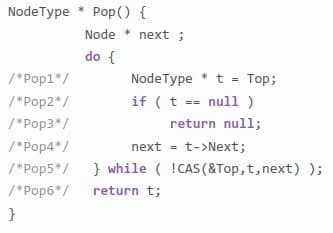
\includegraphics[scale=0.47]{ABA1}
			\end{figure}
		\end{minipage}
		\hfill
		\begin{minipage}[h]{0.64\linewidth}
			\begin{figure}
				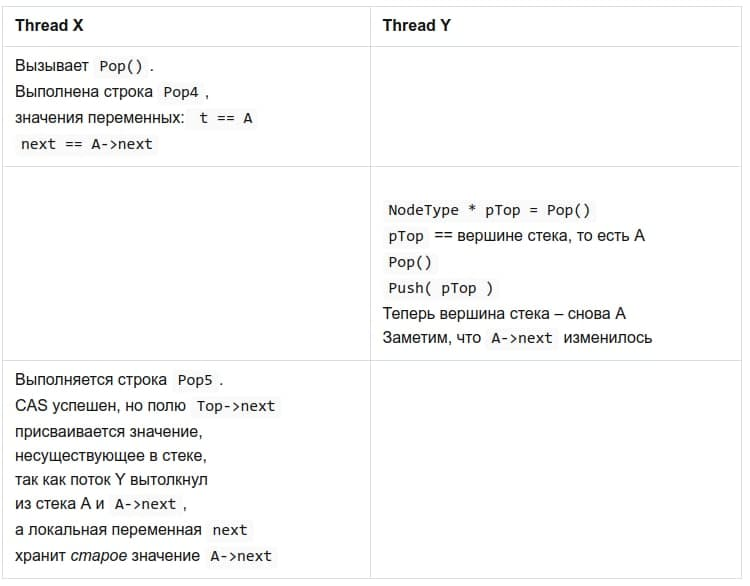
\includegraphics[scale=0.45]{ABA2}
			\end{figure}
		\end{minipage}
		Как бороться? Отложенное удаление
	\end{frame}

	\begin{frame}{Особенности реализации lock-free очереди}
		\begin{itemize}
			\item Общий концепт: пытаться прилинковать новый элемент к очереди в вечном цикле, пока CAS не завершится успехом
			\item Управление двумя указателями с помощью одного CAS (dCAS существуют не во всех реализациях x86-64)
			\item Для решения ABA-проблемы использовать, например, Epoch-based reclamation или Hazard pointer (\href{https://habr.com/ru/post/202190/}{ссылка})
		\end{itemize}
	\end{frame}

	\begin{frame}{Источники}
		\begin{itemize}
			\item M. Herlihy, N. Shavit, The Art of Multiprocessor Programming, Morgan Kaufmann,2008
			\item Э. Уильямс, Параллельное программирование на С++ в действии, ДМК Пресс,2012
			\item \href{https://habr.com/ru/post/195948/}{Атомарные примитивы (кликабельно)}
			\item \href{https://habr.com/ru/post/216013/}{Lock-free стек (кликабельно)}
			\item \href{https://habr.com/ru/post/219201/}{Lock-free очередь (кликабельно)}
		\end{itemize}
	\end{frame}
\end{document}